\section{Sensitivity Analysis in Photodynamics}\label{sec:sensitivity_analysis_in_photodynamics}
\textit{Commentary on: \fullcite{10.1021/acs.jctc.4c01008}}

The first published work of this thesis is focused on sensitivity analysis in photodynamics simulations from article \textit{Sensitivity Analysis in Photodynamics: How Does the Electronic Structure Control \textit{cis}-Stilbene Photodynamics?} in \textit{Journal of Chemical Theory and Computation}. A reaction video to this article by Pavlo O. Dral has been published on YouTube.\supercite{Z4qFv-QZMR8}

In computational photodynamics, nonadiabatic dynamics simulations are becoming standard tools to investigate the excited-state behavior of molecular systems. However, the accuracy of these simulations strongly depends on the chosen electronic structure method used to compute \gls{pes} and \gls{nacv}. Researchers often face the challenge of selecting an appropriate electronic structure method, as different methods often yield varying results for the same system.\supercite{10.1021/acs.jctc.3c00908,10.1021/acs.jctc.2c00968,10.1021/acs.jctc.9b00282} This work exposes this challenge by performing a sensitivity analysis on the photodynamics of \textit{cis}-stilbene, a prototypical photoisomerization system. \textit{cis}-stilbene is a textbook example of a photochemical reaction where the excited wavepacket splits into competing channels: isomerization around its central double bond to form the \textit{trans} isomer (\textit{trans}-stilbene), and photocyclization to form \gls{dhp}. Historically, theoretical studies have yielded contradictory results regarding which of these pathways dominates. This discrepancy arises because the energy balance between the relevant \gls{ci} is highly sensitive to the chosen electronic structure method, making \textit{cis}-stilbene the perfect candidate for this sensitivity analysis. The three isomers are depicted in Fig.~\ref{fig:stilbene_isomers}.
\begin{figure}[!ht]
\centering
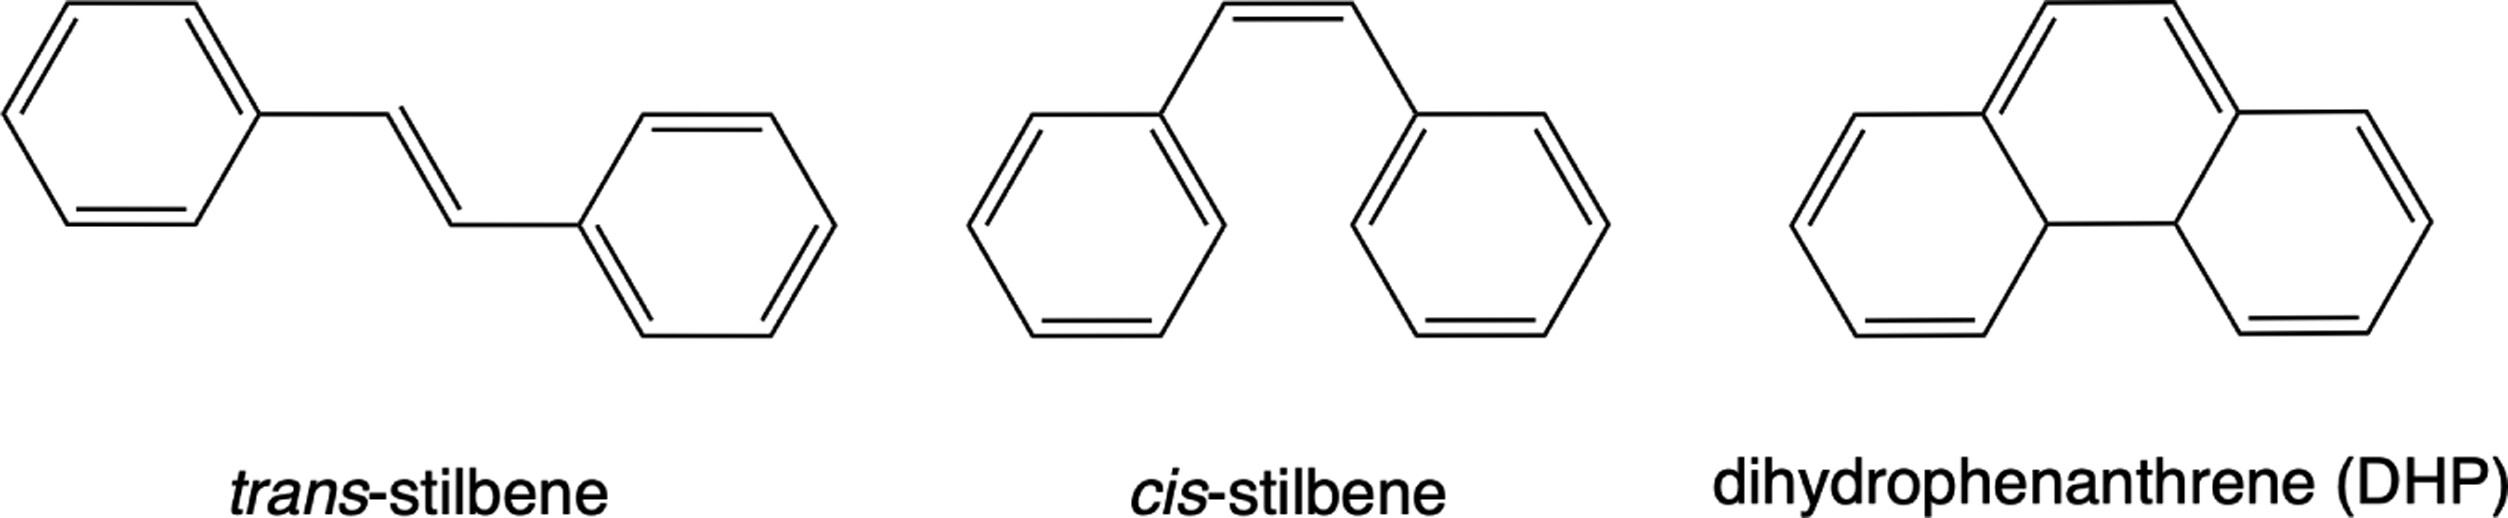
\includegraphics[width=0.9\linewidth]{parts/02-Original_Research_and_Contributions/chapters/02-Primary_Scientific_Contributions/sections/images/images_large_ct4c01008_0001}
\caption{The three stilbene isomers.}
\label{fig:stilbene_isomers}
\end{figure}
The study uses the \gls{fssh} method, described in Sec.~\ref{sec:fewest_switches}, to simulate the nonadiabatic dynamics of \textit{cis}-stilbene using various electronic structure methods. For the low-level method, semiempirical OM3-MRCISD is employed, while for the high-level methods, \gls{sa-casscf} and \gls{sa-caspt2} were used. Using these methods, the study calculates the excited-state lifetimes and populations, quantum yields for photoisomerization and cyclization, and \gls{trpes}. The results are then compared with the experimental data to assess the accuracy of each electronic structure method.
\subsection{Mapping the Potential Energy Surface}
To start the sensitivity analysis, the study first establishes the investigated \gls{pes} and all the important features that influence the photodynamics of \textit{cis}-stilbene. Upon excitation to the first excited state (S$_1$) there are two main relaxation pathways. The first pathway leads through the \textit{cis}-stilbene S$_1$ minimum to an energetically close \gls{ci} between S$_1$ and the ground state (S$_0$) that facilitates the isomerization to \gls{dhp} or back to \textit{cis}-stilbene. The second pathway leads through another S$_1$ minimum to four \glspl{ci} between S$_1$ and S$_0$ that facilitate the isomerization to \textit{trans}-stilbene or back to \textit{cis}-stilbene. Note that all of the \glspl{ci} are energetically accessible from the S$_1$ \gls{fc} region. The \gls{pes} features on all three electronic structure levels are qualitatively similar, with no seemingly preferred pathway. The schematic representation of the \gls{pes} features is shown in Fig.~\ref{fig:pes_features_stilbene}.
\begin{figure}[!ht]
\centering
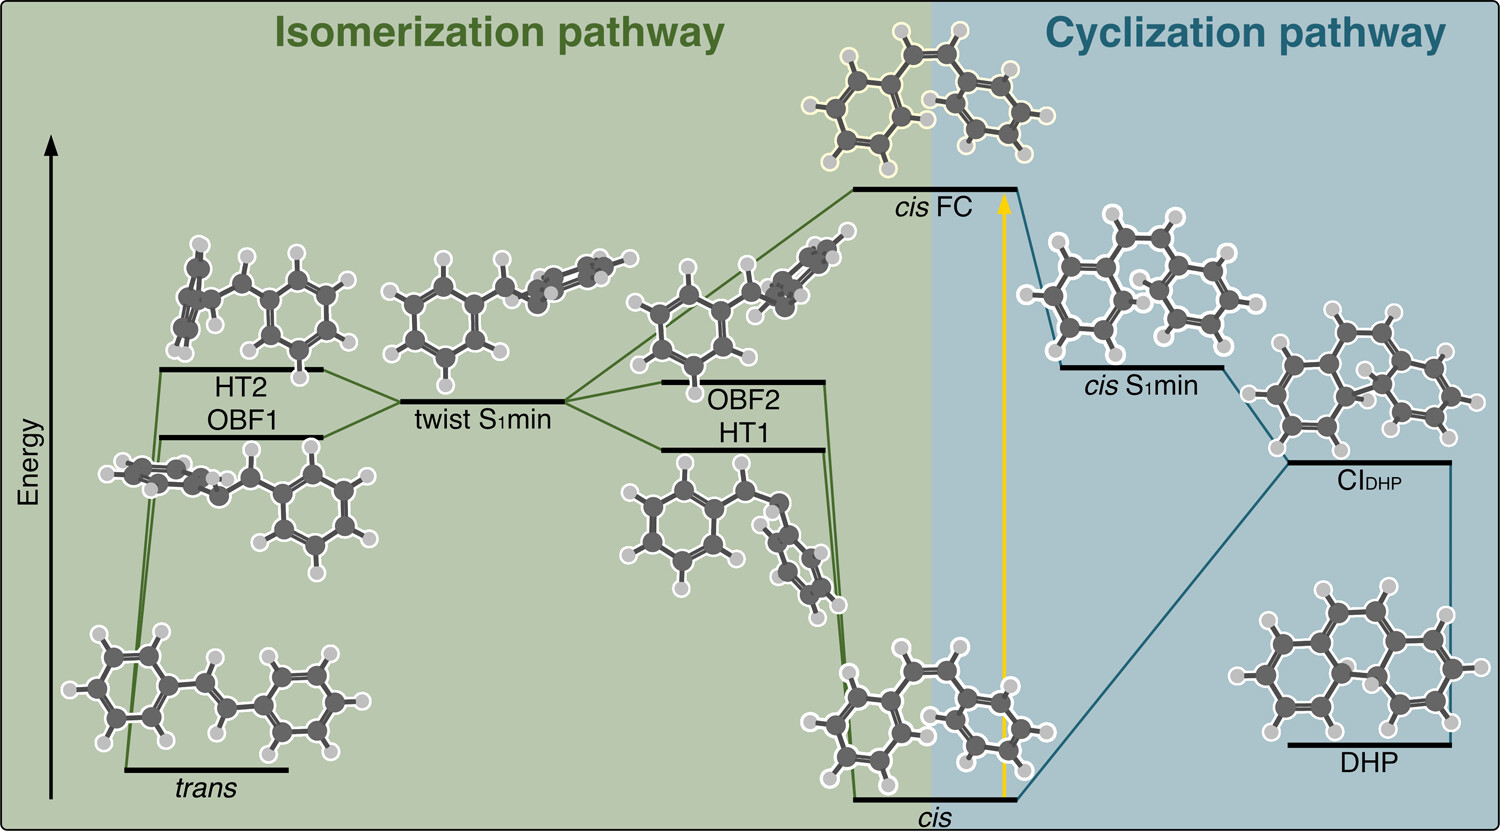
\includegraphics[width=\linewidth]{parts/02-Original_Research_and_Contributions/chapters/02-Primary_Scientific_Contributions/sections/images/images_large_ct4c01008_0003}
\caption{Schematic representation of the \gls{pes} features of \textit{cis}-stilbene relevant to its photodynamics. The diagram illustrates the two main relaxation pathways from the S$_1$ excited state: one leading to the formation of \gls{dhp} via a \gls{ci} accessible from the S$_1$ minimum, and the other leading to \textit{trans}-stilbene via multiple \glspl{ci}.}
\label{fig:pes_features_stilbene}
\end{figure}
\subsection{Nonadiabatic Dynamics Simulations and Results}
After characterizing the stationary points, nonadiabatic dynamics simulations were performed using different electronic structure methods. Quantum yields and excited-state lifetimes obtained from these simulations are summarized in Tab.~\ref{tab:sensitivity_analysis_results}.
\begin{table}[!ht]
\centering
\caption{Summary of the photodynamics results for \textit{cis}-stilbene using different electronic structure methods. The quantum yields for \textit{cis}-stilbene ($\phi_{\symit{cis}}$), \textit{trans}-stilbene ($\phi_{\symit{trans}}$), and \gls{dhp} ($\phi_{\symrm{DHP}}$) formation, along with the excited-state lifetime ($\tau$), are presented. The results from previous studies and experimental data are also included for comparison.}
    \label{tab:sensitivity_analysis_results}
    \begin{tabular}{lcccc}
        \hline
        Level of Theory&$\phi_{\symit{cis}}$&$\phi_{\symit{trans}}$&$\phi_{\symrm{DHP}}$&$\tau$ (fs)\\
        \hline
        OM3-MRCISD(12,17) (LZSH)& $0.48\pm0.05$&$0.52\pm0.05$&$0.00\pm0.00$ &$321\pm10$\\
        SA2-CASSCF/SVP&$0.29\pm0.06$&$0.68\pm0.06$&$0.03\pm0.02$&$360\pm6$\\
        XMS-SA3-CASPT2/cc-pVDZ&$0.55\pm0.14$&$0.02\pm0.04$&$0.43\pm0.14$&$295\pm10$\\
        XMS-SA2-CASPT2/cc-pVDZ&$0.91\pm0.07$&$0.00\pm0.00$&$0.09\pm0.07$&--\\
        \hline
        XMS-SA3-CASPT2(2,2)/cc-pVDZ\supercite{10.1021/jacs.2c12266}&$0.55\pm0.14$&$0.04\pm0.10$&$0.41\pm0.14$& $572\pm16$\\
        OM3-MRCISD(12,17)\supercite{10.1038/s41557-022-01012-0}&0.48&0.52&0.0&$\approx500$\\
        SA2-CASSCF(2,2)/6-31G*\supercite{10.1021/acs.jpcb.0c03344}&$0.45\pm0.04$&$0.52\pm0.04$&$0.04\pm0.01$&$520\pm40$\\
        \hline
        Experiment in Solvents\supercite{10.1021/ja00076a041,10.1021/acs.jpca.8b04011}&0.47-0.59&0.35-0.39&0.05-0.08&380-1650\\
        \hline
    \end{tabular}
\end{table}
The results show significant differences in the quantum yields and excited-state lifetimes depending on the electronic structure method used. The OM3-MRCISD method predicts a nearly equal distribution between \textit{trans}-stilbene and \textit{cis}-stilbene formation, with no \gls{dhp} formation. Whereas the SA2-CASSCF method predicts a higher quantum yield for \textit{trans}-stilbene formation, with a small amount of \gls{dhp} formation. And finally, the XMS-SA3-CASPT2 method predicts a high quantum yield for \gls{dhp} formation, with a low quantum yield for \textit{trans}-stilbene formation. The XMS-SA2-CASPT2 method turns out to be inadequate for describing the photodynamics of \textit{cis}-stilbene, as it predicts almost no population transfer to the ground state. This failure originates from the exclusion of a critical doubly excited state from the state-averaging space. Without the inclusion of this state, the topography of the S$_1$ surface is artificially distorted, creating a deep minimum that traps the wavepacket and prevents it from accessing the \glspl{ci}. Conversely, including this third state in the averaging space (as done in the XMS-SA3-CASPT2 method) corrects the topography, allowing the wavepacket to reach the crossing seams and opening the photocyclization channel.

The excited-state lifetimes also vary, but all methods predict lifetimes comparable to the lower end of the experimental range. The quantum yields in the table above lead to a conclusion that the choice of electronic structure method has a profound impact on the predicted photodynamics. The simple static picture of the \gls{pes} features does not provide enough information to predict the outcome of the dynamics simulations, as all methods show similar \gls{pes} features but yield different photodynamics results.
\subsection{Time-Resolved Photoelectron Spectra}
The study also analyzes the \gls{trpes} obtained from the simulations (Fig.~\ref{fig:stilbene_spectra}) and compares them with experimental data. The \gls{trpes} signal is predominantly sensitive to the initial wavepacket motion out of the \gls{fc} region, rather than the long-time branching ratio at the distant \glspl{ci}. Because all the tested methods (with the exception of the flawed XMS-SA2-CASPT2) predict a very similar initial descent on the S$_1$ surface, their simulated spectra all reasonably match the experimental data. This observation is critical: it demonstrates that agreement with experimental \gls{trpes} alone is insufficient to validate an electronic structure method's ability to accurately predict long-time photoproduct quantum yields.
\begin{figure}[!ht]
\centering
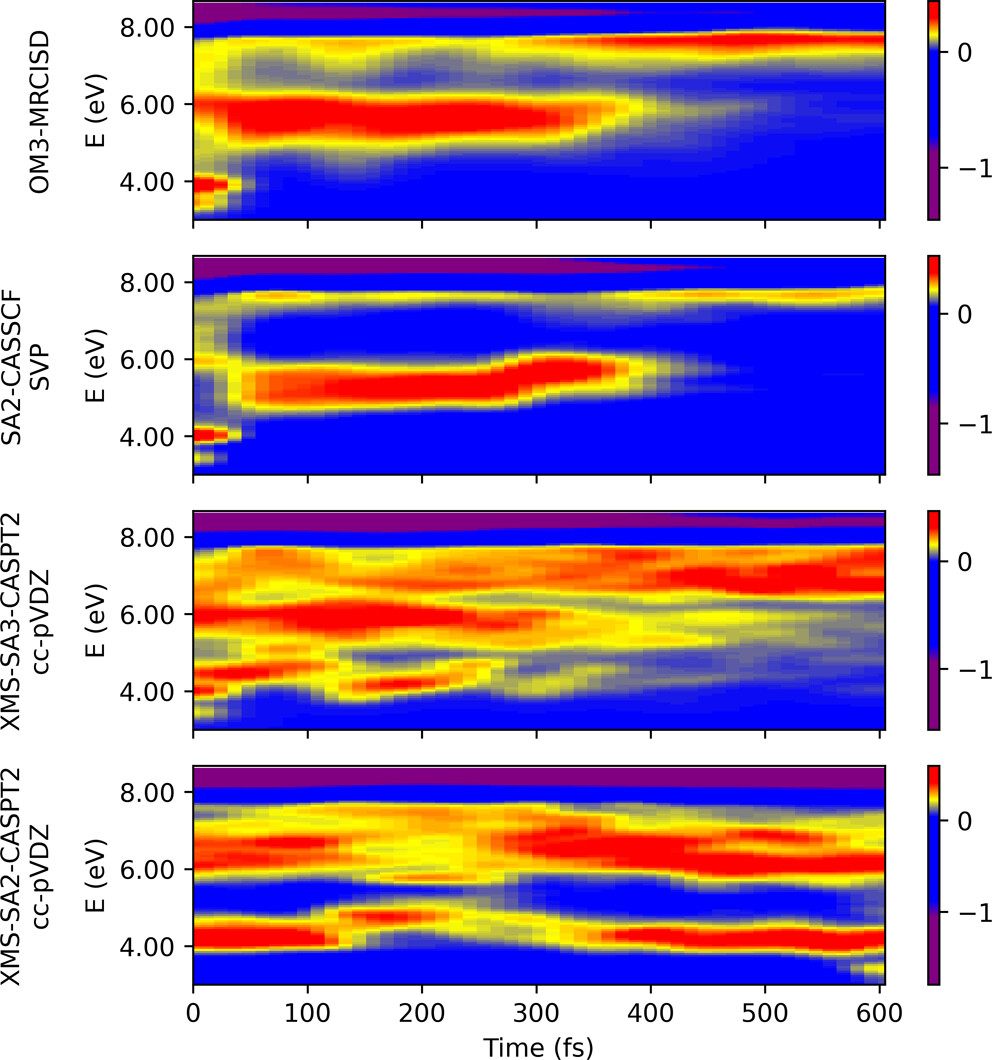
\includegraphics[width=0.7\linewidth]{parts/02-Original_Research_and_Contributions/chapters/02-Primary_Scientific_Contributions/sections/images/images_large_ct4c01008_0009}
\caption{Simulated \gls{trpes} for surface hopping dynamics with various electronic structure methods}
\label{fig:stilbene_spectra}
\end{figure}
Because experimental spectra alone cannot distinguish between various theoretical outcomes, alternative strategies must be utilized to systematically assess the reliability of the underlying electronic structure methods.
\subsection{Nonadiabatic Dynamics Simulations with a Bias Potential}
The drastic differences in quantum yields beg the question: How can we efficiently map the system's sensitivity of nonadiabatic dynamics without the immense computational cost of running trajectories on multiple high-level methods? To explore this, the study introduces an approach where a computationally cheap semiempirical method (OM3-MRCISD) is artificially perturbed to mimic the topographic shifts seen in higher-level methods. 

Specifically, an artificial harmonic bias potential $V_{\text{bias}}=\frac{1}{2}k(r_{ce}-r_{eq})^2$ was added to the central \ce{C=C} bond distance $r_{ce}$, where $k$ is a variable force constant and $r_{eq}$ is the equilibrium bond length. By tuning $k$, the relative energies of the \glspl{ci} can be systematically shifted with respect to the \gls{fc} region without completely recalculating the electronic structure.
\begin{figure}[!ht]
\centering
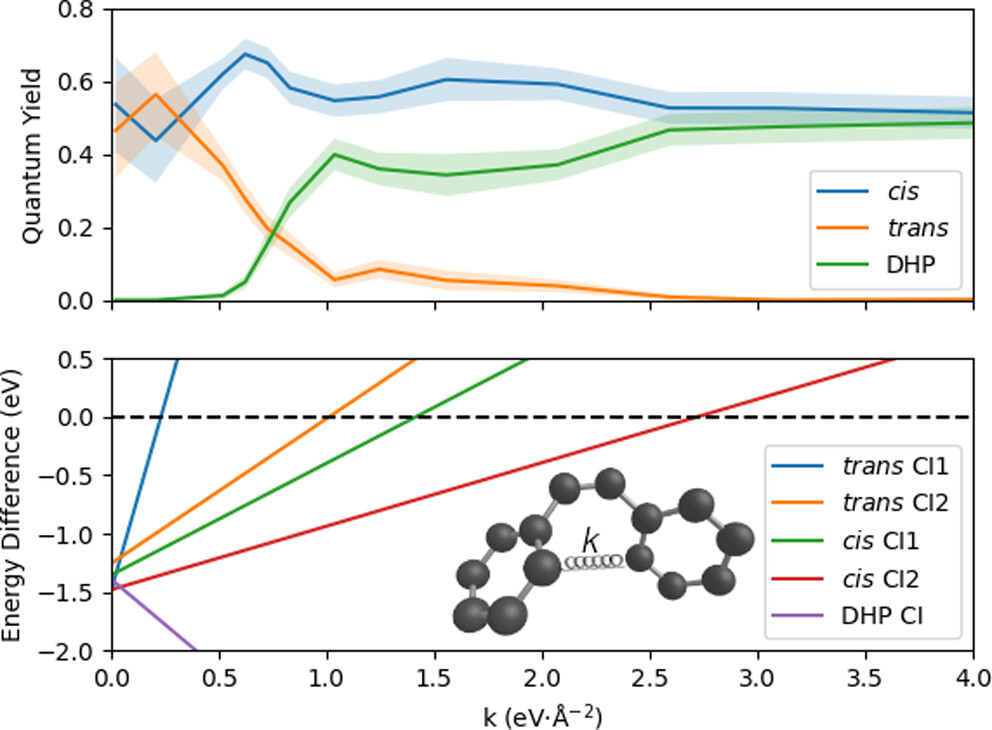
\includegraphics[width=0.7\linewidth]{parts/02-Original_Research_and_Contributions/chapters/02-Primary_Scientific_Contributions/sections/images/images_large_ct4c01008_0011}
\caption{Quantum yields of \textit{cis}-stilbene photoproducts as a function of applied force constant. The upper panel shows the product ratio on the force constant $k$ of the harmonic oscillator, as referenced in the paragraph above. The lower panel shows the energy difference between the \gls{fc} point (dashed line) and several \glspl{ci}, also varying with different values of $k$.}
\label{fig:stilbene_oscillator}
\end{figure}
As shown in Fig.~\ref{fig:stilbene_oscillator}, altering the force constant $k$ directly manipulates the energetic accessibility of the competing pathways. Increasing $k$ effectively raises the energy barrier toward the \textit{trans} pathway. Consequently, the wavepacket is redirected, shifting the population flow to heavily favor the cyclization pathway and yielding more \gls{dhp}. This cleanly demonstrates that even minor energetic shifts on the \gls{pes} can completely invert the macroscopic quantum yields of the reaction.
\subsection{Conclusion}
The investigation of \textit{cis}-stilbene photodynamics demonstrates that the choice of electronic structure method can drastically alter the long-time photoproduct distributions, even when the underlying \gls{pes} features appear qualitatively similar. We learned that the reproducing the short-time dynamics and \gls{trpes} is not sufficient to validate the method's ability to predict the long-time quantum yields. The initial descent from the \gls{fc} region is similar across methods, leading to similar \gls{trpes}, but the branching ratios at the distant \glspl{ci} are highly sensitive to the shape of the \gls{pes} and can vary drastically between methods. By introducing an additional bias potential, we were able to systematically explore how small energetic shifts can completely invert the photoproduct distributions.

In the broader context of this dissertation, these findings emphasize the absolute necessity of algorithmic benchmarking and numerical validation in nonadiabatic dynamics simulations. This work successfully bridges the gap between the purely theoretical analysis of mixed quantum-classical algorithms, as performed in Sec.~\ref{sec:coherence_in_mixed_qc_dynamics}, and the practical application of these algorithms to realistic, highly sensitive photochemical systems.

These findings highlight a critical vulnerability in standard theoretical photochemical workflows. As nonadiabatic dynamics simulations are becoming increasingly common, researchers must be wary of relying on a single comfortable electronic structure method without thorough validation or validating their method solely based on short-time observables. The bias potential approach introduced in this work provides a simple yet powerful tool for assessing the sensitivity of photodynamics outcomes to \gls{pes} features without the need for high-level \textit{ab initio} calculations. By adopting such analyses, the community can gain deeper insights into the relationship between electronic structure and photodynamics, ultimately leading to more reliable predictions and a better understanding of complex photochemical processes.
